\begin{question}
\noindent Triangle $P$ and triangle $Q$ are shown on the grid below.

\begin{center}
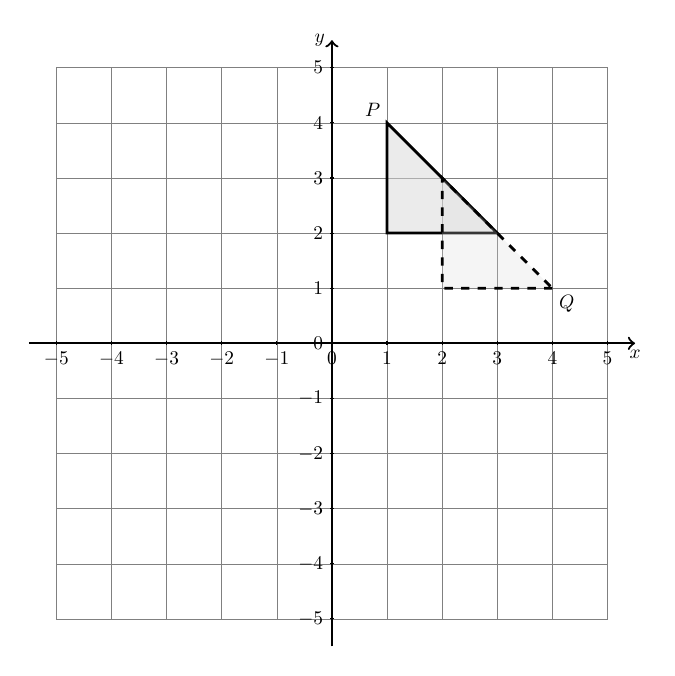
\begin{tikzpicture}[scale=0.7, transform shape]
    % Define colours
    \definecolor{borderColour}{HTML}{000000}
    \definecolor{fillColour}{HTML}{D8D8D8}

    % Define axis scale
    \def\axisLimit{5}

    % Draw grid
    \draw[step=1cm,gray,very thin] (-\axisLimit,-\axisLimit) grid (\axisLimit,\axisLimit);

    % Draw axes
    \draw[thick,->] (-\axisLimit-0.5,0) -- (\axisLimit+0.5,0) node[anchor=north] {$x$};
    \draw[thick,->] (0,-\axisLimit-0.5) -- (0,\axisLimit+0.5) node[anchor=east] {$y$};

    % Label x-axis and y-axis
    \foreach \x in {-\axisLimit,...,\axisLimit}
        \draw (\x cm,1pt) -- (\x cm,-1pt) node[anchor=north] {$\x$};
    \foreach \y in {-\axisLimit,...,\axisLimit}
        \draw (1pt,\y cm) -- (-1pt,\y cm) node[anchor=east] {$\y$};

    % Define coordinates for triangle P
    \coordinate (A) at (1,4);
    \coordinate (B) at (1,2);
    \coordinate (C) at (3,2);

    % Draw triangle P
    \filldraw[fill=fillColour, draw=borderColour, line width=1pt, fill opacity=0.5] (A) -- (B) -- (C) -- cycle;

    % Label the vertices of triangle P
    \node[above left] at (A) {$P$};

    % Define coordinates for triangle Q (reflection in y = x)
    \coordinate (A') at (4,1);
    \coordinate (B') at (2,1);
    \coordinate (C') at (2,3);

    % Draw triangle Q
    \filldraw[fill=fillColour, draw=borderColour, line width=1pt, fill opacity=0.25, dashed] (A') -- (B') -- (C') -- cycle;

    % Label the vertices of triangle Q
    \node[below right] at (A') {$Q$};

\end{tikzpicture}
\end{center}

\noindent Triangle $Q$ is the image of triangle $P$ after a single reflection.

\noindent Find the equation of the mirror line.
\vspace{4cm}
\begin{flushright}
    \answerplain{3}
\end{flushright}
\end{question}
